\chapter{Podstawy teoretyczne}
\section[Symulacja komputerowa][Symulacja komputerowa]{Symulacja Komputerowa}

\subsection{Wstęp}
\par{
Ludzkość od zarania dziejów stara się analizować otaczający ją świat. Nie bez powodu. Zrozumienie zasad wg. funkcjonuje otaczająca nas rzeczywistość zdaje się znacząco ułatwiać naszą egzystencję co w prostej linii prowadzi do tego, że samo dążenie do zgłębienia prawideł świata da się wytłumaczyć odwołując się bezpośrednio do ewolucji - osobniki lepiej rozumiejące otaczający świat potrafią lepiej się mierzyć z pojawiającymi się w nim przeciwnościami.
}

\par{
Zasadniczo ludzkie badania działają na dwóch płaszczyznach - dążą do przewidywania przyszłości i pozwalają podejmować coraz lepsze reakcje na bieżące zdarzenia.
}

\par{
Przez wiele lat ludzie prowadzili rozliczne badania starające się wyjaśniać naturę świata - z początku nieco chaotycznie (co nie znaczy, że bez znaczących sukcesów) - u zarania nauki w starożytnej Grecji, gdy cała nauka zamknięta była w jedną dziedzinę nazywaną ogólnym mianem Filozofii.
Wraz z rozwojem ludzkości nasze podejście do nauki jako takiej ewoluowało. I tak już w XVII wieku Kartezjusz wysuwał postulaty, że podstawą nauki powinny być pewne abstrakcyjne narzędzia jak matematyka i logika na bazie których buduje się teorię innych dziedzin. Współczenie niewiele odsuneliśmy się od myśli Kartezjusza - podstawą naszych badań zdaje się być matematyka, na którą nakładane są inne dziedziny jak fizyka i chemia, których wypadkową są nauki przyrodnicze.
}

\par{
Warto zwrócić uwagę, że nasza nauka układa się wsosób warstwowy - kolejne warstwy pozwalają nam odcinać się od reguł obowiązujących w małej skali i budować torie dla skali większej. Jest to szczególnie uzasadnione w świetle odkryć XX wieku, jak ogólna teoria względności.
}

\par{
Oczywiście nadal wiele naukowych tez ma charakter czysto empiryczny i często jest to wystarczające dla określonych zastosowań - w końcu po dziś dzień nauka służy ludziom a nie odwrotnie.
}

\par{
Mamy więc doczynienia z pozornym rozłamem nauki - z jednej strony formalizmy pozwalające na precyzyjny, spójny i co najważniejsze - jednoznaczny, opis określonych zjawisk. Z drugiej strony badania empiryczne, na podstawie których często wyszukuje się potencjalnych dróg rozwoju w sposób analityczny. Obie te metody uzupełniają się wzajemnie - niektórych badań praktycznych nie sposób zaplanować bez określonych reguł i znajomości niektórych torii a jednocześnnie niektóre teorie (w zasadzie większość) nie powstały by gdyby nie konkretne obserwacje rzeczywistości.
}

\par{
Symulacja komputerowa, zdaje się być odpowiedzią na drugą metodykę, która jednakowoż ściśle wykorzystuje specyficzny aparat matematyczny. Stosując ją wykorzystujemy bowiem teorie w pewnej skali, by odtworzyć zachowania i obserować ich skutki w innej (zwykle większej), np. symulując ruch cząsteczek cieczy wg. określonych fizyką zasad by obserwować zachowanie cieczy jako całości w określonych warunkach.
}

\par{
Czym jest więc symulacja komputerowa? Symulacja to proces, który pozwala przy użyciu reguł jednej skali obserwować zjawiska w innej. Słowo komputerowa odnosi się do konkretnej realizacji - z wykorzystaniem maszyn cyfrowych. Dobrym podsumowaniem ukazującym funkcję symulacji komputerowej zdaje się być poniższy schemat przedstawiający trzy filary współczesnej nauki wg. prof. Michała Kleibera.
\begin{center}
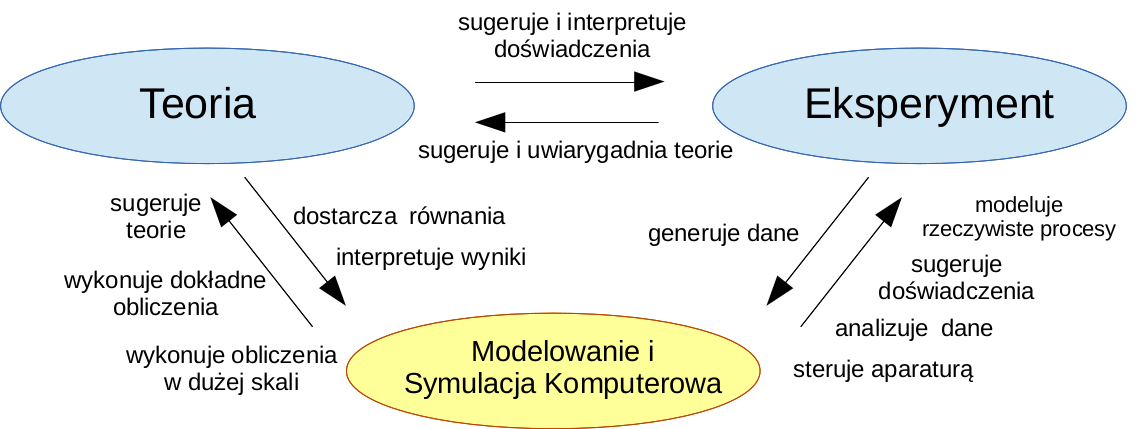
\includegraphics[width=\textwidth,keepaspectratio]{img/triada_poznania}
\textit{Trzy filary poznawcze współczesnej nauki [5].}
\end{center}
}

\subsection{Filozofia symulacji komputerowej}

\subsubsection{Postulat Laplace'a}
\par{
W roku 1814 Pierre Simon Laplace opublikował \textit{Essai philosophique sur les probabilites} (fran. \textit{Filozoficzny esej na temat prawdopodobieństwa}), w którym wysunął następujący postulat:
}
\par{
\textit{Umysł, który by znał siły działające w danej chwili w przyrodzie oraz wzajemne położenie wszystkich istotności, z których ona się składa, gdyby zdołał ująć je i poddać analizie - w jednym wzorze zawarłby ruchy największych ciał niebieskich i najdrobniejszych atomów. Nie byłoby dla niego nic niepewnego i zarówno przyszłość, jak i przeszłość świata byłyby obecne dla jego oka ...
}}
\par{
\textit{... Jesteśmy tak dalecy od chwili, kiedy poznamy wszystkie siły przyrody i różne formy ich oddziaływania, że nie byłoby godnym filozofa negowanie pewnych zjawisk jedynie dlatego, że nie można ich objaśnić przy obecnym stanie wiedzy. Jesteśmy zobowiązani do badania zjawisk tym dokładniej, im trudniej przychodzi nam uznać je za istniejące.}
}

\par{
Współczesna nauka odsunęła się nieco od tej koncepcji. Po pierwsze przyjmuje się (mając na względzie zasady fizyki kwantowej), że świat nie opiera sie o deterministyczne zasady - co w zasadzie obala postulat Laplace'a. Po drugie nastomiast, zgodnie z zasadą nieoznaczoności Heisenberga [7] nie jest możliwe uzyskanie pełnego obrazu świata ponieważ każda jego obserwacja wpływa na jego stan - co uniemożliwia wykorzystanie postulatu Laplace'a w praktyce.
}
\par{
Obalenie teorii Laplace'a nie oznacza bynajmniej, że nie pozostaje ona poza światem nauki - nadal ma ona bardzo duże znaczenie filozoficzne oraz nadal aktualna pozostaje jej druga część. Ponadto, w wielu sytuacjach zakłada się, że zasada ta nadal obowiązuje - jednym z takich miejsc jest symulacja komputerowa.
}
\par{
Podstawą w zasadzie każdej symulacji komputerowej jest stan symulowanych obiektów oraz oddziaływania między nimi. Zakłada się, że symulator zna \textbf{wszystkie} zasady obowiązujące w symulowanym świecie jak i stan wszystkich obiektów w nim występujących i w związku z tym jest w stanie określić przyszłość symulowanego układu - jest to stan, o którym wspominał Laplace'a, a symulator można by w tym kontekście potraktować jako demona Laplace'a. Warto zwrócić uwagę, że w podejściu takim nie ma nic zdrożnego, ani sprzecznego ze współczesną nauką - przedewszystkim dlatego, że ograniczenie symulacji do ciągu przyczyn i skutków nie obniża zwykle jej wartości w kwestii celu jaki się przed nią stawia.
}

\subsubsection{Precyzja komputerów}
\par{
Kolejnym problem w pewien sposób uniemożliwający przyrównanie rzeczywstości do symulacji komputerowej jest fakt, że współczesne komputery przechowują dane w sposób skwantowany (binarny). W związku z tym nie sposób opisać na nim danych o charakterze ciągłym z dowolną precyzją.
}
\par{
Choć zdawać by się mogło, że w świetle współczesnych badań, ograniczenie to przestaje mieć sens, ponieważ przyjmuje się, że wszelkie zjawiska w przyrodzie mają charakter kwantowy, to należy wziąć pod uwagę jak małe są kwanty o których mówi ta teoria.
}
\par{
Długość Plancka (czyli minimalna obserwowalna we wrzechświecie odległość) wyniosi 
\begin{center}
$l_P = c \ t_P = \sqrt{\frac{\hbar G}{c^3}} = 1,616 199(97) \times 10^{-35} m$
\end{center}
co oznacza, że aby zapisać na komputerze dokładne położenie obiektu w trójwymiarowej kostce o boku długości jednego metra potrzebowali byśmy ok. $3.5 \times 10^{65}$ terabajta pamięci. Przy obecnej technologii zdaje się więc, że dokładność komputera jest zasadniczym problemem uniemożliwiającym dokładne odwzorowanie rzeczywistości.
}

\subsubsection{Praktyczne znaczenie ograniczeń}
\par{
W praktyce, wyżej wymienione ograniczenia nie są zwykle krytyczne. Zazwyczaj bowiem symulacja ma za zadanie upraszczać wygląd rzeczywistości, a więc nadmierna precyzja jest w wręcz niewskazana.
}
\par{
Warto jednak zdawać sobie sprawę, że symulacja komputerowa jest jedynie pewnym przybliżeniem rzeczywistości i z samej swojej natury obarczona jest zasadniczym błędem - i własnie \textbf{znalezienie takiego sposobu symulacji by błąd w możliwie małym stopniu wpływał na aspekty istotne z punktu widzenia celu symulacji zdaje się być istotą jej projektowania.}
}

\subsection{Zastosowanie symulacji}

\subsubsection{Przewidywanie zdarzeń}
\par{
Podstawowym zdaniem stawianym przed symulacjami komputerowymi zdaje się być przewidywanie różnego rodzaju zdarzeń. Znając zasady wg. których funkcjonują pewne zjawiska, jesteśmy w stanie do pewnego stopnia określić jak będą rozwijały się te zjawiska w przyszłości.
}
\par{
Niektóre z tych zjawisk potrafiliśmy przewidywać już przed erą symulacji komputerowej - albo przy użyciu klasycznego aparatu matematycznego albo przy użyciu własnej intuicji i doświadczenia. Jednak symulowanie zjawisk w celu przewidywania ich rozwoju przenosi przewidywanie przyszłości na zupełnie nowy poziom.
}
\par{
Na symulację możemy wpływać - tj. sprawdzać jak będzie reagowała na poszczególne bodźce ze świata zewnętrznego. Możemy także sterować jej przebiegiem - tj. w miejscach gdzie pojawia się niepewność związana z metodyką symulacji wybrać konkretny wariant rozwiązania problemu.
Dzięki temu, jesteśmy w stanie, w którkim czasie wytworzyć i przeanalizować wiele sceneriuszy wydarzeń i na podstawie tych doświadczeń podejmować działania (w szczególności realne działania prewencyjne).
}
\par{
Przykładem tego rodzaju zastosowań jest symulowanie przebiegu huraganu, pozwalające przewidywać jego rozwój, kierunek i szybkość przemieszczania się w zależności od licznych, często samych w sobie trudnych do przewidzenia okoliczności. Na podstawie tego rodzaju symulacji uruchamia się służby kryzysowe w odpowiednich rejonach, informuje się mieszkańców o zagrożeniu, czy zarządza ewakuację.
}

\subsubsection{Badania i eksperymenty}
\par{
Drugi typ zastosowań ma ścisły związek z badaniami naukowymi.
Opisując model pewnych zjawisk, przy użyciu symulatora jesteśmy w stanie sprawdzać reakcję całego układu na naszą ingerencję jak i obserwować jego zachowanie w stanie zamkniętym. Tego rodzaju badanie może często uzmysławiać pewne zjawiska w innej skali, niż ta na której rozpatrywany jest układ w modelu symulacji.
}
\par{
Przeprowadzanie niektórych eksperymentów w świecie realnym jest często problematyczne, kosztowne lub wręcz niemożliwe. Symulowanie eksperymentów zdaje się pozwalać w znacznym stopniu usprawniać badania a także wskazywać kierunki dalszego rozwoju. Jednocześnie najbardziej udane eksperymenty często powtarza się w rzeczywistości by uzyskać bardziej precyzyjny i pewny obraz.
}
\par{
Przykładem zastsowania w tym sektorze może być np. symulacja zbiornika z wodą na poziomie pojedyńczych cząsteczek by symulować jej zachowanie w konkretnych sytuacjach (np. uderzenie). Mając do dyspozycji taki symulator możemy zaobserować jak reaguje tafla wody na uderzenie i np. wysnuć teorię na temat związku długości fali na wodzie z siłą uderzenia.
}

\subsubsection{Testowanie}
\par{
Często spotykanym problemem, na który napotykają inżynierowie jest niemożność testowania ich rozwiązań w realnych warunkach. W takich sytuacjach z pomocą często przychodzą komputerowe symulacje. Dostarczają one danych do badań, lub pozwalają obserwować reakcje układu na działanie wdrażanego systemu.
}
\par{
Symulator opisywany w niniejszej pracy został stworzony z myślą o właśnie takim zastosowaniu. Ma on za zadanie generować dane wyjściowe dotyczące ruchu w środowisku miejskim przeznaczone jako wejście dla systemu śledzenia obiektów, który przystosowany został do pracy z realnymi danymi.
}
\par{
Rozwiązanie wykorzystujące symulator jest tańsze, szybsze oraz znacznie prostsze i może w znacznym stopniu wyprzedzać bieżące czasy.
Zebranie realnych danych na temat pojazdów poruszających się po mieście jest zadaniem nie łatwym. Kamery z funkcją rozponawania obiektów są dopiero raczkującą technologią a ich umieszczenie w całym mieście jest bardzo kosztowne. Umieszczenie ludzi spisujących odpowiednie, jest mało precyzyjne, i obarczone innym rodzajem błędów niż odczyty z kamer. Uzyskanie realnych danych potrzebnych do testowania skuteczności systemu śledzenia zdaje się więc być praktycznie niemożliwe.
}
\par{
Z pomocą przychodzą symulatory - za ich pomocą możemy wytworzyć takie dane, jakich powinna nam dostarczyć hipotetyczna kamera. Nałożyć na nie odpowiednie szumy. I zapisać razem z o wiele szerszymi danymi realnymi pozwalającymi analizować skuteczność wykorzystanych rozwiązań.
}
\par{
Dzięki temu, praca nad systemami śledzenia może postępować niezależnie od prac nad systemami monitoringu. Takie podejście sprawia że w sytuacji stworzenia i wdrożenia odpowiedniej realnej bazy sprzętowej będzie istniało już gotowe oprogramowanie mogące w pełni wykorzystać jej możliwości.
}
\par{
Wykorzystanie symulatorów do testowania zdaje się pozwalać na oszczędzanie dużej ilości zasobów i może prowadzić do skrócenia czasu badań pozwalając na unikanie kłopotliwych przygotowań do realnego testowania w trakcie koncepcyjnego opracowywania projektowanego systemu.
}

\subsubsection{Wizualizacja (także interaktywna)}
\par{
Ostatnim, acz nie najmniej istotnym z zastosowań symulatorów jest tworzenie wizualizacji w tym wizualizacji interaktywnych.
}
\par{
Organoleptyczne przekazywanie informacji jest bardzo istotne z punktu widzenia funkcjonowania człowieka - dane dostarczone w sposób nieprzetworzony są zwykle niezrozumiałe lub wymagają dużych nakładów czasu by wyciąganąć z nich potrzebne informację. Ponieważ często symulator ma za zadanie zaprezentować ogólny pogląd na symulowane zjawisko, typowo wraz z symulatorem dostarczany jest system pozwalający zwizualizować jego pracę.
}
\par{
Praktyczne zastosowanie tego rodzaju tandemu zdaje się być bardzo szerokie. Pozwala to na prezentowanie sedna złożonych zjawisk, ułatwia przekazywania informacji, pozwala na obserwowanie zjawisk, do których odruchowej analizy człowiek jest całe życie przyzwyczajany. Dzięki temu często w sposób heurystyczny jesteśmy w stanie wyznaczyć pewne prawidłowości, których zasadność często sprawdzana jest dokładnie albo analitycznie albo z wykorzystaniem tego samego symulatora i dołączonego do niego modułu analizującego dane.
}
\par{
Prezentując dane przy użyciu odpowiedniej wizualizacji, jesteśmy w stanie przekazać złożone informacje w sposób intuicyjnie zrozumiały. Jest to cenna właściwość szczególnie dla edukacji czy wszelkiego rodzaju ciał doradczych współpracujących z podmiotami nie operującymi naukową nomenklaturą.
}
\par{
Powołując się ponownie na przykład symulacji cząstek wody by obserować ich powierzchnię, wynikiem takiego symulatora było by zapewne położenie poszczególnych cząstek wody. Jednak chcąc widzieć realną powierzchnię - często z uzyskanych danych wytworzymy trójwymiarowy obraz dający nam wrażenie jakbyśmy pracowali z realną cieczą.
}
\par{
Wizualizowanie wszelkich zjawisk zdaje się być nierozłącznie związane z ich symulowaniem i stanowi istotny element a w wielu sytuacjach cel egzystencji symulatorów jako takich.
}

\subsection{Model symulacji komputerowej}
\subsubsection{Definicja modelu}
Modelem w symulacji komputerowej nazywamy zasady, wedle których funkcjonuje symulacja, uwzględniający wszelkie zmienne wejściowe i wyprowadzający z nich zmienne wyjściowe z uwzględnieniem upływu czasu.
\par{
W literaturze [3] można spotkać następującą, nieco bardziej ścisłą definicję:
Model \textit{to operator przekształcający zadane zmienne wejściowe X(t) w zmienne wyjściowe Y(t) czyli 
\begin{center}
$Y(t) = H_{t} \times X(t).$
\end{center}
}
}.

\subsubsection{Oczekiwane cechy modelu}
\par{
Przed modelami do symulacji najczęściej stawiane są trzy wymagania [2,4]:
\begin{itemize}
\item Wymaganie jednoznaczności - oznacza to, że operator modelu jest zależnością funkcyjną tzn. że jeden zbiór danych wejściowych daje dokładnie jedną odpowiedź.
\item Wymaganie spójności (rozwiązywalności) - oznacza to, że elementy modelu nie przeczą sobie nazajem (są matematycznie spójne).
\item Wymaganie stabilności - wymaganie to, oznacza, że niewielkie zmiany danych wejściowych nie powinny pociągać za sobą gwałtownych zmian w danych wyjściowych. Należy jednak zwrócić uwagę, iż niekiedy symulowany system posiada właściwości przeczące tej zasadzie - nietrudno wyobrazić sobie na przykład symulację nacisku na jakiś obiekt, który po przekroczeniu pewnej krytycznej wartości siły nacisku łamie się, powodując diametralną zmianę wyglądu całego systemu (w wyniku reakcji łancuchowej). 
\end{itemize}
}

\subsection{Taksonomia modeli}
\par{
Literatura [2,3,4] podaje wiele kryteriów podziału modeli, poniżej zestawiono najbardziej ostre spośród nich.
}

\subsubsection{Podział ze względu na istnienie czasu}
\par{
\begin{itemize}
\item model dynamiczny - znacznie bardziej popularny, upływ czasu jest uwzględniany w modelu i ma wpływ na wartości zmiennych wyjściowych.
\item model statyczny - nie uwzględnia upływu czasu lub wartosci zmiennych wyjściowych nie zależą od niego w żaden sposób.
\end{itemize}
}

\subsubsection{Podział ze względu na model czasu}
\par{
Dotyczy tylko modeli dynamicznych.
\begin{itemize}
\item model ciągły w czasie - istnieje możliwość wyznaczenia wartości parametrów wyjściowych dla dowolnej chwili czasowej.
\item model dyskretny w czasie - istnieje możliwość wyznaczenia wartości parametrów końcowych tylko dla przeliczalnego zbioru chwil czasowych.
\end{itemize}
}

\subsubsection{Podział ze względu na determinizm}
\par{
\begin{itemize}
\item model deterministyczny - dla danego stanu początkowego daje zawsze taki sam wynik.
\item model niedeterministyczny - wynik działania modelu nie jest zdetermininowany w momencie zadania stanu wejściowego.
\end{itemize}
}
\par{
Warto mieć na względzie, że modele niedeterministyczne niejako stoją w sprzeczności z postulatem Laplace'a jak i z postawionym wyżej wymaganiem jednoznaczności. Należy jednak pamiętać, że w typowym przypadku narzędziem programistycznym dla symulacji operującej na modelu niedeterministycznym będzie symulator liczb pseudolosowych, który choć wykazuje cechy probabilistyczne charakterystyczne dla liczb losowych, w rzeczywistości bazuje na deterministycznych zdarzeniach - w praktyce więc każda komputerowa implementacja symulatora będzie miała charakter deterministyczny.
}

\subsubsection{Podział ze względu na oddziaływanie ze światem zewnętrznym}
\par{
\begin{itemize}
\item model autonomiczny - tworzy zamknięty układ i nie uwzględnia żadnych możliwości interakcji z jego zewnętrzem.
\item model nieautonomiczny - pozwala na dostarczanie bodźców (pobudzeń, wartości) z zewnątrz, które mają wpływ na zmienne wyjściowe.
\end{itemize}
}

\subsubsection{Podział ze względu na rodzaj związków między wejściem a wyjściem}
\par{
\begin{itemize}
\item model liniowy - zmienne wyjściowe są związane ze zmiennymi wejściowymi przy użyciu liniowych funkcji.
\item model nieliniowy - wykorzystuje funkcje nieliniowe do obliczania wartości parametrów wyjściowych.
\end{itemize}
}

\subsubsection{Podział ze względu na sposób tworzenia}
\par{
\begin{itemize}
\item model dedukcyjny - reguły modelu pochodzą na podstawie teorii opisującej modelowane zjawisko.
\item model empiryczny - reguły są tworzone na podstawie obserwacji zachowań modelowanego zjawiska, tak by model miał podobne obserwowalne właściwości.
\end{itemize}
}

\subsection{Modelowanie}
\par{
Proces tworzenia modeli pewnych zjawisk (np. na potrzeby symulacji komputerowej) nazywany jest modelowaniem. Proces ten, stanowi często wyzwanie dla przystępujących do niego inżynierów ze względu na bardzo wysokość złożoność zagadnień jak i konieczność dobierania miejsc, które model będzie upraszczał względem rzeczywistości, tak by zachować zasadność tworzenia modelu.
}

\subsubsection{Aspekty tworzenie modeli}
\par{
Przystępując do modelowania jakichkolwiek zjawisk poprawnym podejściem jest zwrócenie uwagi na następujące aspekty [2]:
\begin{itemize}
\item \textbf{cel} - celowi tworzenia modelu powinny być podporządkowane wszystkie związane z nim działania. Należy pamiętać, że to model istnieje dla celu a nie odwrotnie. Cel symulacji stanowi punkt odniesienia, do którego należy często powracać i podporządkowywać mu decyzje podejmowane podczas modelowania.
\item \textbf{poziom uproszczenia} - model z samej swojej natury musi być pewnym uproszczonym odpowiednikiem wycinka rzeczywistości. Jego stopień skomplikowania nie może być zbyt wysoki, przez względ na dostępne metody praktycznej implementacji symulacji oń opertej. Z drugiej strony wybranie modelu nadmiernie uproszczonego moze prowadzić do zagubienia pewnych specyficznych zachowań symulowanego zjawiska - co może fałszować obraz symulacji. Dobrym określeniem porządanego stopnia uproszczenia modelu mogą być słowa Alberta Einsteina: \textit{Wszys­tko po­win­no być tak pros­te, jak to tyl­ko możli­we, ale nie pros­tsze.}
\item \textbf{potrzeby eksperymentu} - niezywkle często zdarza się, że zjawisko modelowane jest z zamiarem wykorzystania do ściśle określonego eksperymentu. Mając taką świadomość, jesteśmy w stanie łatwiej dobrać możliwe uproszczenia, a co ważniejsze pozbyć się wielu niepotrzebnych zależności z proponowanego modelu.
\item \textbf{poprawność} - model uznaje się za poprawny, jeśli poddany każdemu możliwemu wejściu zachowa się wystarczająco podobnie do realnego zjawiska poddanego bodźcom odpowiadającym temu wejściu. Określenie, czy dane wyjście jest wystarczająco podobne do wyjścia realnego jest decyzją jaką podejmuje modelujący mając na względnie różne aspekty modelu a w szczególności cel jego tworzenia. Zależności jakie powinny zachodzić w poprawnym modelu przedstawia poniższy rysunek.
\par{
\begin{center}
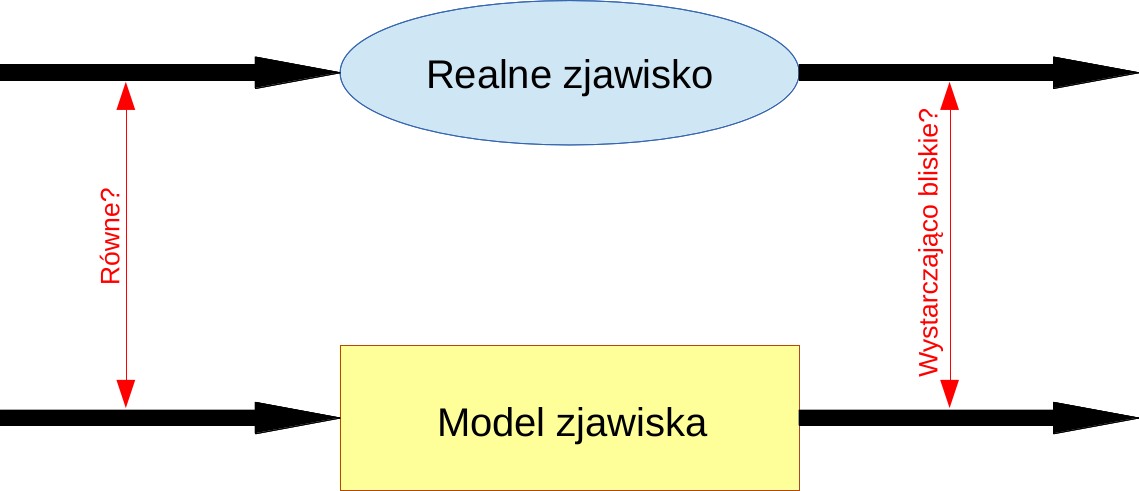
\includegraphics[width=\textwidth,keepaspectratio]{img/poprawnosc_modelu}
\textit{Popraność modelu względem modelowanego zjawiska [2].}
\end{center}
}
\item \textbf{przydatność} - model uznawany jest za przydatny gdy jego złożoność rośnie wolniej niż wykładniczo względem ilości zmiennych wykorzystywanych do jego opisu [2]. Modele zagadnień o złożoności wykładniczej mogą być poprawne, jednak ich precyzyjny opis jest często nieprzydatny i wymagane jest ich uproszczenie, by rozwiązywać symulowane zagadnienie z mniejszą dokładnością (np. heurystycznie) ale ciągle wystarczająco dobrze z punktu widzenia symulacji a jednocześnie w realnie dostępnym czasie.
\item \textbf{wiarygodność} - wiarygodność modelu określa na ile użytkownik jest przekonany o jego poprawności, szczególnie bazując na obserwacji wyników jego działania i organoleptycznym porównaniu tych wyników z realnym zjawiskiem. Wiarygodność modelu jest szczególnie istotna w przypadku symulacji przeznaczonych do wizualizacji określonych zjawisk.
\end{itemize}
}

\subsubsection{Zasadność modelu}
\par{
Model jako taki musi posiadać pewne cechy by był przydatny do jakichkolwiek zastosowań. Zastosowanie wyżej sformułowanych kryteriów doboru, powinno zapewnić, że model będzie właściwie sformułowany, jednak warto mieć dodatkowo na względzie dwa aspekty, wedle których można ocenić zasadność istnienia zaproponowanego przez nas modelu [4].
\begin{itemize}
\item Badanie modelu nie powinno być bardziej złożone od badanie właściwego zjawiska.
\item Model powinien (zwłaszcza w kwestiach związanych ze swoim celem) zachowywać się w sposób zbliżony do modelowanego zjawiska.
\end{itemize}
}


\section[Podstawy fizyczne][Podstawy fizyczne]{Podstawy fizyczne}

\subsection{Fizyczne modele dynamiki Newtona}
\par{
Do stworzenia odpowiedniego modelu symulacji komputerowej, oprócz znajomości metodyki modelowania wymagana jest znajomość teorii stojącej za modelowanym zjawiskiem oraz aparatu matematycznego dla niej odpowiedniego.
Ruch obiektów w środowisku miejskim jest związany ściśle z klasyczną dynamiką Newtona. W fizyce klasycznej funkcjonują dwa podstawowe modele uproszczone opisujące ruch obiektów wg. zasad dynamiki Newtona - model bryły sztywnej i punktu materialnego.
}

\subsubsection{Dynamika bryły sztywnej}
\par{
Model bryły sztywnej uwzględnia kształt i wymiary obiektu poruszającego sie w przestrzeni. Jego podstawą jest założenie, że każdy obiekt ma strukturę jednostajnej, sztywnej (niezmieniającej kształtu pod względem czynników zewnętrznych) oraz nie absorbującej energii bryły, która poddawana jest wszelakim oddziaływaniom.
}
\par{
W związku z tym, że model bryły sztywnej zakłada wymiarowość obiektów, posiadają one w tym modelu sześć stopni swobody, które określają ich położenie w trójwymiarowej przestrzeni:
\begin{itemize}
\item Trzy związane z ruchem postępowym
	\begin{itemize}
	\item szerokość (położenie na osi X)
	\item wysokość (położenie na osi Y)
	\item głębokość (położenie na osi Z)
	\end{itemize}
\item Trzy związane z ruchem obrotowym
	\begin{itemize}
	\item Kąt roll (obrót wokół osi X)
	\item Kąt yaw (obrót wokół osi Y)
	\item Kąt pitch (obrót wokół osi Z)
	\end{itemize}
\end{itemize}
}
\par{
\begin{center}
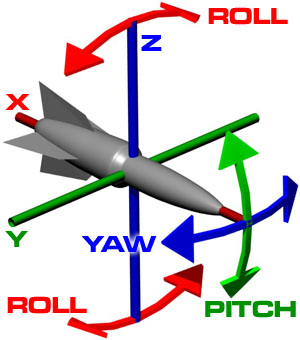
\includegraphics[]{img/xyz_ryp}
\end{center}
}
\par{
\begin{center}
\textit{Stopnie swobody bryły szytwnej, źródło: $http://www.projectrho.com/public\_html/rocket/controldeck.php$}
\end{center}
}
\subsubsection{Dynamika punktu materialnego}
\par{
Model punktu materialnego nie uwzględnia kształtu i fizycznego charakteru poruszającego się w przestrzeni ciała. W tym modelu przyjmuje się, że ciało (a więc cała masa) skupione jest w przestrzeni o zerowych wymiarach (punkcie). Tego rodzaju uproszczenie znacząco obniża skomplikowania rachunków związanych z ruchem ciał, jednak uniemożliwa rozpatrywanie ich ruchu obrotowego jak i nie jest w stanie bez dodatkowego wsparcia zapewnić spójnego opisu zderzeń obiektów (dwa punkty nie mogą się zderzyć gdyż nie mają wymiarów).
}

\par{
Ponieważ punkt materialny nie ma wymiarów, posiada zaledwie trzy stopnie swobody, związane z położeniem, nie jest natomiast opisywany przez obroty (jak bryła sztywna):
\begin{itemize}
\item szerokość (położenie na osi X)
\item wysokość (położenie na osi Y)
\item głębokość (położenie na osi Z)
\end{itemize}
}

\subsection{Rozwiązywanie równań dynamiki}
\par{
Posiadanie modelu fizycznego i odpowiedniej bazy matematycznej dla danego zjawiska pozwala na jego wykorzystanie, jednak wszelkie obliczenia związane z symulacją komputerową odbywać się będą przy użyciu maszyn cyfrowych. Koniecznym jest więc znalezienie sposobów numerycznego rozwiązywania problemów charakterystycznych dla wybranego modelu fizycznego - w tym wypadku dynamiki punktu materialnego.
}

\section[Systemy fuzji danych][Systemy fuzji danych]{Systemy fuzji danych}
\par{
\textit{Fuzją danych} nazywa się [14] \textit{proces łączący dane w celu oczyszczenia estymaty i predykcji stanu.}, który jest uogólnieniem wcześniejszej definicji [13] mówiącej, że \textit{Fuzja danych to proces obsługujący asocjację, korelację i wiązanie ze sobą danych i informacji z jednego lub wielu źródeł w celu uzyskania lepszej pozycji i tożsamości obiektu oraz możliwie trafnej i precyzyjnej ocenie sytuacji i zagrożenia.}.
}
\par{
Obie powyższe definicje zdają się oddawać kwintesencję fuzji danych, którą jest zbieranie wielu danych o niedużej wartości jednostkowej w celu uzyskania szerokiego obrazu o dużej wartości końcowej.
}

\subsection{Rodzaje fuzji}
\par{
Systemy fuzji danych dzieli się ze względu na charakter danych poddawanych obróbce. Fuzją \textbf{danych} nazywa się procesy wykorzystujące dane pozbawione wstępnej obróbki lub ograniczające wstępną obróbkę do wyrównania dziedzin danych pochodzących z różnych źródeł. Systemy fuzji danych operują na danych nieprzetworzonych np. właściwościach fizycznych sygnałów analogowych.
}
\par{
Bardziej rozpowszechniona od fuzji danych jest fuzja \textbf{informacji} nazywana również fuzją \textbf{cech} lub fuzją \textbf{właściwości} --- operująca na danych obrobionych mających znaczenie na wyższym poziomie abstrakcji. Przykładem tego rodzaju systemu może być system operujący na danych dostarczanych z inteligentnych kamer w środowisku miejskim - analizujący konkrente informacje o znanym charaketrze (np. położenie obiektu) w celu uzyskania szerszych informacji na jego temat (np. śledzenie jego pozycji w czasie).
}
\par{
Rzadziej spotykanymi ale także wymienianymi w literaturze [15] są systemy fuzji \textbf{decyzji}. O tym przypadku mówi się, kiedy przetwarzanie danych przed samą fuzją dochodzi jeszcze o krok dalej - tzn. na podstawie danych przed fuzją wypracowywana jest pewna decyzja. W takim przypadku dopiero niezależne decyzje z wielu źródeł są łączone w celu wypracowania rozwiązania ogólnego. Oznacza to, że daną w takim rozumieniu jest jakaś zmienna o charakterze sterującym sama sobie będąca wnioskiem z dostarczonych informacji, natomiast zadaniem systemu fuzji jest wybranie sumarycznej decyzji systemu nie wnikając w wewnętrzne funkcjonowanie poszczególnych swoich części a jedynie w poddecyzje.
}
\par{
Kolejne stopnie przetworzenia danych o których mowa powyżej można by przedstawić na podstawie systemu fuzji danych mającego dawać werdykt w kwestii zwycięscy wyborów prezydenckich w Stanach Zjednoczonych Ameryki. System, dla którego danymi wejściowymi były by zdjęcia wypełnionych kart do głosowania byłby w takim ujęciu systemem fuzji danych. Wstępne przetworzenie danych, np. przez odczytanie informacji z kart do głosowania lub wręcz dostarczenia sum wyników z poszczególnych lokali wyborczych zaprowadziło by nas do systemu, mogącego zakrawać na system fuzji informacji. Jeśli jednak poszli byśmy krok dalej i zebrali tego rodzaju informacje dla każdego stanu z osobna i na tej podstawie wyznaczyli decyzję w postaci preferowanego przez dany stan prezydenta, a następnie przesłali tę decyzję do systemu, który decydował by o końcowym wyborze, mieli byśmy doczynienia z syntezą decyzji. W rzeczywistości system głosowania w stanach zdjednoczonych jest właśnie złożeniem tych trzech warstw.
}
\par{
Da się wyraźnie dostrzec, że poszczególne typy fuzji różnią się stopniem obróbki danych przed wejściem do systemu. W związku z tym systemy fuzji danych wydają się być bardziej złożone ale jednocześnie tracące najmniejszą ilość informacji. Zastosowane konkrentego rodzaju fuzji zależy ściśle od dzidziny zastosowania i intencji twórcy systemu - nie sposób jest poszeregować wyników poszczególnych typów systemów w kategorii lepszy-gorszy.
}
\subsection{Model JDL}
\par{
Lata doświadczeń nad systemami fuzji danych pozwoliły na wypracowanie pewnych wzorców ich funkcjonowania stanowiących swoise ramy dla wszystkich nowych systemów. Ilość modeli powstałych w czasie badań jest zuważalnie duża, jednak większość z nich zdaje się być jedynie szczególnym przypadkiem modelu zwanego modelem JDL.
}
\par{
Model JDL dzieli proces fuzji danych na pięć poziomów:
\begin{itemize}
\item \textbf{Poziom 0, preprocessing} --- na tym poziomie dokonuje się wstępnego przygotowania danych otrzymanych z zewnątrz systemu. Dane mogą być wyrównane do spójnej dziedziny czy jednostek, zagregowane względem określonych cech itd. Każda obróbka tego rodzaju może następować również poza systemem więc zasadność występowania tego poziomu zależy od tego jak bardzo porządany przez nas rodzaj wejścia różni się od tego dostarczanego do systemu.
\item \textbf{Poziom 1, asocjacja} --- faza ta odpowiada za łączenie ze sobą danych pochodzących z różnych źródeł. Uwzględnia ona modele dotyczące obiektów w systemie pozwalając na estymację stanu obiektów na podstawie połączonych danych z wielu źródeł.
\item \textbf{Poziom 2, ocena sytuacji} --- na tym poziomie na podstawie ogólnych zasad funkcjonowania znanych już w momencie tworzenia systemu wyciągane są wnioski dotyczące jego bieżącego stanu.
\item \textbf{Poziom 3, ocena wpływu} --- na podstawie wyników poprzednich poziomów, zarówno bieżących jak i historycznych poziom ten stara się estymować przyszły stan obiektów. Poziom ten odpowiada również za interpretację wyników estymacji w szczególności wykrywając pewne sceneriusze jako potencjalnie nietypowe, niebezpieczne lub po prostu wymagające reakcji.
\item \textbf{Poziom 4, decyzje} --- zadaniem ostatniej fazy jest reagowanie na określone zdarzenia w systemie fuzji obserwowalne przez pryzmat poprzednich poziomów. Zapewnia to sprzężenie zwrotne, tzn. sam system fuzji danych zaczyna wpływać na obserwowane zjawiska a jednocześnie stanowi swoistą kwintesencję sensu istnienia tego rodzaju systemów zwłaszcza w ich pierwotnym znaczeniu.
\end{itemize}
}
\par{
Model JDL ma pochodzenie militarno-wojskowe. Został on opracowany przez Data Fusion Subpanel of the Joint Directors of Laboratories (JDL) w 1985 roku [16]. W związku z tym nomenklatura używana do jego opisu jak i cele jakie stawia się przed tym modelem są ściśle związane z potrzebami wojskowymi. Nic jednak nie stało na przeszkodzie żeby wykorzystać tę metodykę w zastosowaniach cywilnych czego przykładem może system DAFNE implementujący dwa pierwsze poziomy modelu JDL [17]).
}
\par{
\begin{center}
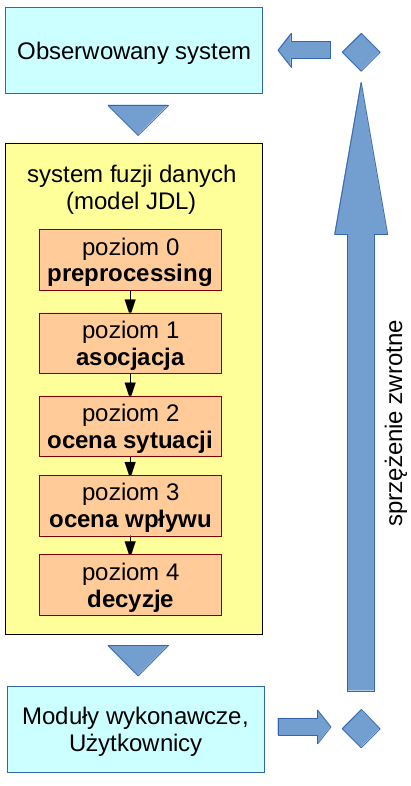
\includegraphics[width=15em,keepaspectratio]{img/jdl}
\end{center}
}
\par{
\begin{center}
\textit{Działanie systemu fuzji danych w modelu JDL}
\end{center}

\subsection{System śledzenia}
\par{
Opis modelu JDL stanowi jedynie podstawowę dla dalszych rozważań dotyczących konkrenych systemów fuzji danych, pokazuje on jednak generalną logikę stojącą za systemami fuzji niezależnie od metodyki i linii podziału tej logiki na konkrene warstwy.
}
\par{
System śledzenia, dla celów którego tworzony jest opisywany w pracy symulator, jest typowym systemem fuzji informacji. Ma on za zadanie zbierać informacje z wielu czujników rozmieszczonych w środowisku miejskim i na ich podstawie wyznaczać trasy poszczególnych obiektów a także przewidywać dlasze kierunki ich poruszania sie.
}
\par{
Z puntku widzenia takiego systemu podstawową informacje dotyczącą obiektów i poddawaną fuzji stanowi położenie obiektu, jednakże system ten zakłada możliwość dostarczania przez czujniki większej ilości informacji i może w przyszłośći wykorzystywać je by zwiększać swoją skuteczność.
}
\par{
Takie wymagania systemu ciągną za sobą faktyczne znaczenie postawienia pracy w kontekście systemów fuzji. Oznacza to bowiem, że system ten \textbf{musi} dostarczać dla docelowego systemu informacji w formie wstępnie przetworzonej dotyczącej położenia obiektów obserwowanych przez inteligentne czujniki oraz, że te czujniki \textbf{mogą} dostarczać większej ilości informacji.
}
\par{
Ponieważ wyżej zaprezentowany ogólny wstęp dotyczący systemów fuzji danych pozwolił na sformułowanie tego zagadnienia w kontekście pracy a same systemy fuzji nie są przedmiotem tej pracy, nie będą one bardziej szczegółowo opisywane.
}

\section[Elementy symulowanego środowiska][Elementy symulowanego środowiska]{Elementy symulowanego środowiska}
\par{
Środowiskem miejskim nazywa się tu ogół obiektów znajdującej się w czterowymiarowej przestrzeni w otoczeniu ludzkich miast, powiązanych wzajemnymi relacjami. Elementami środowiska miejskiego są więc piesi i chodniki, pojazdy i ulice, budynki i ich mieszkńcy, parki wraz z lokalną fauną i florą czy post industrialne ruiny ozdobione dzikimi wysypiskami śmieci.
}
\par{
Środowisko miejskie rysuje się więc jako bardzo kompleksowe pojęcie, które nie sposób modelować w całej rozciągłości. Jednakże, z punktu widzenia systemów dozoru czy też śledzenia wystarczającym wydaje się być przedstawienia całego środowska miejskiego jako zbioru obiektów niżej wymienionych typów. Należy pamietać, że poniżej zaproponowany podział nie jest jedynym możliwym, a został wybrany do omówienia ponieważ pozwalał na jednocześnie na zaprezentowanie samego środowiska jak i płynne przejście do jego modelowania w dalszej części pracy.
}
\subsection{Obiekty statyczne}
\par{
Obiektami statycznymi w środowisku miejskim nazywamy wszystkie elementy krajobrazu niezmienne w czasie ale posiadające fizyczną reprezentację, mogącą wchodzić w pośrednią lub bezpośrednią interakcję z innymi obiektami.
}
\par{
W wypadku przestrzeni czterowymiarowej, jaką jest środowisko miejskie, każdy obiekt posiadający fizyczną reprezentację w naturalny sposób opisywany jest bryłą potencjalnie zmienną w czasie. Jako że obiekty statyczne z samej swojej natury są niezmienne w czasie są one opisywane trójwymiarową bryłą o określonej pozycji w trzech wymiarach i znajdująca się w tej pozycji w każdym punkcie wymiaru czwartego (czasu).
}
\par{
Poza reprezentacją w formie bryły każdy element tego rodzaju może być opisywany w całości lub częściami rozmaitymi parametrami mającymi fizyczny wpływ na inne obiekty z otoczenia jak np.
\begin{itemize}
\item Gęstość lub komplementarna masa
\item Przepuszczalność światła
\item Współczynnik odbicia
\item Współczynnik tarcia
\item itd.
\end{itemize}
}
\par{
Ilość uwzględnianych właściwości obiektów statycznych zależy od potrzeb tworzonego modelu. Opisywanie poszczególnych własności fizycznych obiektów nie jest przedmiotem tej pracy. Przy tworzeniu ogólnego modelu dla środowiska miejskiego należy jednak uwzględnić fakt, że tego rodzaju właściwości istniają i w zasleżności od potrzeb konkretnych badań lista uwzględnianych parametrów może być zmienna.
}
\par{
Przykładami obiektów statycznych są:
\begin{itemize}
\item Budynki
\item Roślinność
\item Znaki drogowe
\item Ulice, chodniki
\end{itemize}
}
\subsection{Ścieżki}
\par{
Ulice, chodniki czy inne szlaki po których typowo poruszają się obiekty w środowisku miejskim są określane wspólnym mianem scieżek. Choć ścieżki same w sobie mają zwykle niezmienną w czasie reprezentacje fizyczną, czyli są obiektami statycznymi, to mają one dodatkowe charakterystyczne znaczenie semantyczne.
}
\par{
Ścieżka wyznacza parametryzowalny szlak, po którym mogą poruszać się obiekty pewnego rodzaju. Wyznaczenie tego rodzaju ścieżek zdaje się być typowe dla obserwatorów rzeczywistego świata stąd też specjalne wyróżnienie tego bytu w specjalną grupę.
}
\par{
Wyróżnienie ścieżek ma również praktyczne znaczenie w badaniach - ścieżki wraz z ich semantyką można bowiem w prosty sposób badać pod względem cech związanych z przepływem i umiejscowieniem na nich obiektów.
}
\subsection{Czujniki}
\par{
Jednym z najistotniejszych elementów opisywanego środowiska jest zdolność obiektów w nim się znajdujących do autonomicznego obserwowania stanu swojego otoczenia. W szczególności wszelkiego rodzaju czujniki stanowiące źródło danych dla docelowego systemu fuzji są w stanie zaobserować conajmniej część  spośród cech posiadanych przez obiekty w systemie.
}

\subsubsection{Obserwacja środowiska}
\par{
Środowisko miejskie niezależnie od zastosowanego modelu można potraktować jako zbiór informacji (stan) wraz z opisem zasad jego zmian w czasie. Cały stan układu jest maksymalną informacją niesioną przez system. Choć fakt, ten wydaje się naturalny rozpatrując pozbiór informacji dostarczany do poszczególnych czujników warto mieć na względzie, że zawsze będzie on jedynie podzbiorem lub wynikową podzbioru stanu układu.
}

\subsubsection{Stopień przetworzenia danych}
\par{
Rozpatrując charakter czujników należy przedewszystkim skupić się na uwzględnieniu jakie informacje z modelu mogą one uzyskać. Mogą one mieć dwojaki charakter:
\begin{itemize}
\item Bezpośredni - czujniki odbierają bezpośrednio wielkości znane z modelu środiwska. Tego rodzaju czujniki są zawsze uproszczeniem, ponieważ sam model jest jedynie przybliżeniem rzeczywistości, ale jednocześnie pozwalają na szybkie uzyskanie określonych informacji o określonych cechach systemu, kiedy sam sposób ich pozyskania nie jest przedmiotem badań. Przykładem takiego czujnika może być inteligentna kamera, która dostarcza bezpośrednio odczytów dotyczących pozycji zaobserwowanych obiektów.
\item Fuzyjny - czujniki odbierają informację jako wynik analizy określonych czujników stanowiący syntezę wielu elementów modelu. Zwykła kamera obserwująca kolejne obrazy będące wypadkową kolejnych stanów modelu jest właśnie takim czujnikiem.
\end{itemize}
W przypadku systemu mającego służyć generowaniu konkretnych informacji jakim jest opisywany w tej pracy symulator typowym zdaje się być zastosowanie czujników o charakterze fuzyjnym, co jednakowoż nie przekreśla szansy zastąpienia ich czujnikami fuzyjnym wraz analizatorem ich obserwacji by uzyskać podobne informacje wynikowe w sposób bardziej zbliżony do rzeczywistego.

\subsubsection{Dokładność pomiarów}
\par{
Wszsystkie rzeczywiste obserwacje obarczone są pewnym nieredukowalnym błędem [7]. Naturalnie wymuszony błąd wyniający z praw fizyki nie jest kluczowy z punktu widzenia realnych obserwacji w makroskali, jednak narzędzia do obserwacji w makroskali są obarczone licznymi błędami wynikającymi z ich konstrukcji, szumów analogowych, losowych zdarzeń, które same w sobie nie muszą być modelowane itp.
}
\par{
Centralne twierdzenie graniczne [?], mówi, że suma zmiennych o rozkładach charakteryzujących się taką samą wartością oczekiwaną i wariancją upodabnia się do rozkładu normalnego o takich właście parametrach. Praktycznym wnioskiem wynikającym z tego twierdzenia, jest fakt, że stosowanie rozkładu normalnego przy sztucznym generowaniu błędów jest statystycznie poprawną metodą zepewniającą dla dużej ilości zaszumionych pomiarów zbliżenie do realnych błędów, które zwykle mają cechy zbliżone do warunków postawionych w twierdzeniu. Wydaje się być to poprawne podejście zarówno w przypadku zaszukiania obserwacji bezpośredniej jak i fuzyjnej.
}

\subsection{Obiekty dynamiczne}
\par{
Najważniejszymi z punktu widzenia systemu inwigilacji czy dozoru obiektami są obiekty dynamiczne, ponieważ to właśnie one są obiektem bezpośredniej obserwacji.
}
\par{
Obiekty dynamiczne są reaktywnymi elementami wchodzącymi w interakcje z otoczeniem i mogącymi potencjalnie podejmować autonomiczne decyzje dotyczące zmiany własnego stanu. Podobnie jak obiekty statyczne, obiekty dynamiczne mają swoją reprezentację fizyczną w postaci prametryzowalnej bryły.
}
\par{
W środowisku miejskim wyróżnia się dwie najważniejsze grupy obiektów dynamicznych, których przedstawicie są do siebie zbliżeni pod względem pewnych parametrów.
}
\subsubsection{Pojazdy}
\par{
Pojazd w rozumieniu ruchu drogowego definiowany jest jako obiekt fizyczno-psychiczny [6]. W praktyce bowiem pojazd traktuje się jako tandem pojazd-kierowca (ang. Driver-Vehicle-Element DVE [6]). Tak jak sam pojazd jest faktycznie odzwierciedleniem fizycznej egzystencji DVE w przestrzeni, tak kierowca odpowiada za jego bieżący stan.
}
\par{ }
\par{
\textbf{Kierowca}
}
\par{
Zadaniem kierowcy w tandemie pojazd-kierowca jest podejmowanie decyzji na podstawie obserwowalnych przez niego właściwości otoczenia. W tym znaczeniu, kierowca jest charakterystycznym rozdzajem czujnika, który nie tylko obserwuje pewne własności otocznia ale także podejmuje na ich podstawie decyzje.
}
\par{
Do kierowcy docierają pewne obarczone błędami informacje z zewnątrz (podobnie jak do czujnika), z których na podstawie reguł decyzyjnych wyprowadzane są bieżące akcje polegające na obsłudze interfejsu samochodu (kierownica, pedały itd.). Stworzenie samych reguł decyzyjnych jest zagadanieniem związanym z tworzeniem sztucznej inteligencjii znacznie przewyższającym złożonością zakres tej pracy, i w związku z tym nie będzie tu poruszane. Jednakże, pewne istotne właściwości zachowań ludzkiego kierowcy zostaną tu omówione by wskazać jakie cechy powinny posiadać systemy decyzyjne mające modelować jego działanie.
}
\par{
Podstawowym elementem związanym z reakcjami ludzkimi jest \textbf{czas reakcji}. Czas reakcji składa się z dwóch elementów składowych. Czasu od zdarzenia do rozpoznania konieczności reakcji oraz refleksu czyli czasu jaki upłynie od rozpoznania konieczności reakcji do reakcji mięśniowej [9].
}
\par{
Pierwszy z tych czasów wynosi statystycznie około $0.7s$ [9]. Drugi natomiast ok. $0.25-0.3s$ [9,10] (bardziej precyzyjny rozkład na wykresie poniżej).
}
\par{
\begin{center}
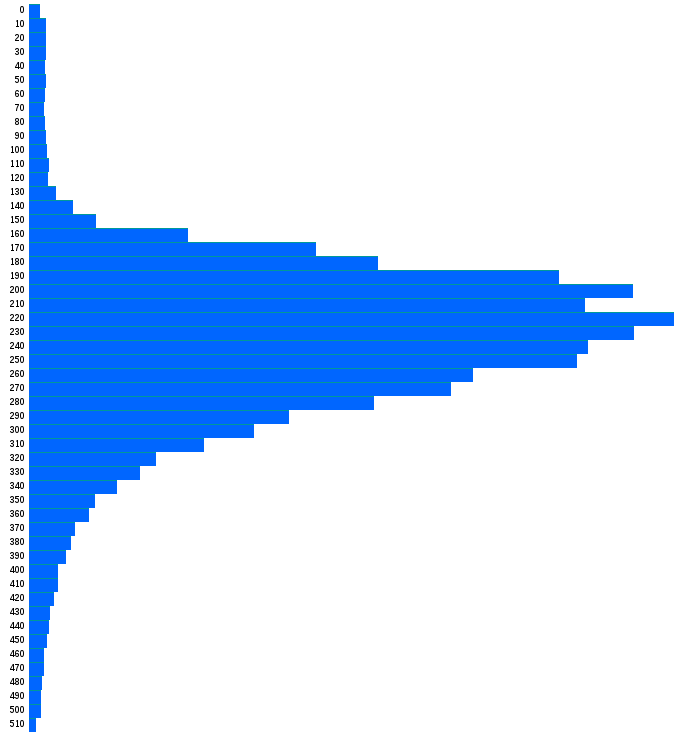
\includegraphics[width=\textwidth,keepaspectratio]{img/reaction_times}
\textit{Rozkład czasu refleksu (ms) [10].}
\end{center}
}
\par{
Sumaryczny czas reakcji wynoszący ok. 1s oznacza w przypadku samochodu poruszającego się z prędkością 50km/h przejechanie ok. 14m. Jest to wielkość obserwowalna i istotna w makroskali w związku z tym wydaje się, że w większości wypadków nie należy zaniedbywać czasu reakcji kierowcy przy budowaniu jego modelu.
}
\par{
Innym istotnym aspektem służacym budowie realnego modelu, choć nie koniecznie niezbędnym do statystycznych badań w typowym przypadku są \textbf{błędy kierowcy}, które zdają się być nieuniknione gdy mamy doczynienia z czynnkiem ludzkim. Błędy kierowcy to przedewszystkim:
\begin{itemize}
\item Błędna ocena sytuacji - np. błędna estymacja czasu dojazdu do skrzyżowania.
\item Błędna reakcja - np. zbyt mocne skręcenie kierownicy.
\item Rozproszenie - np. niedostrzeżenie zagrożenia.
\item Spowolniona reakcja - np. w wyniku spożycia alkoholu.
\end{itemize}
}
\par{
Naturalnym elementem szczególnie w kontekście uwzględnienia przez psychikę kierowcy możliwości wystąpienia jego własnych błędów jest \textbf{uwzględnienie poziomu bezpieczeństwa} przez kierującego. Osoba kierująca samochodem uwzględnia ryzyko jakie niesie jazda w określony sposób i nie zakłada swojej idealnej jazdy.
}
\par{
Kolejnym aspektem, na który zwraca uwagę kierowca jest \textbf{ograniczona wiedza} - często kierowca musi podejmować decyzje nie mając ze względu na pewne ograniczenia (np. widoczności) pełnej wiedzy na temat ruchu w jego okolicy i podejmuje decyzje uwzględniając niejako automatycznie ryzyko związane z wybraniem określonego scenariusza jako domniemanego.
}
\par{
Innym elemnetem związanym z typową jazdą jest zasada \textbf{ograniczonego zaufania}, która mówi o tym, że nie należy ufać w poprawny czy też bezpieczny sposób reagowania pozostałych uczestników ruchu. Konsekwencją tego, jest np. fakt, że kierowaca realnie rusza ze świateł gdy kierowca przed nim zacznie ruszać a nie gdy zobaczy zielone światło. Ma to istotny i nieunikniony wpływ na generalne spowolnienie ruchu.
}
\par{
Kierowca nie decyduje się na jazde z określoną prędkością biorąc pod uwagę ryzyko jakie niesie za sobą zderzenie i inne wydarzenia na drodze. Kierowcą kierują też względy społeczno-ekonomiczne gdy jedzie zgodnie lub niezgodnie z \textbf{przepisami ruchu drogowego}. Niekiedy tylko konieczność dostoswania prędkości czy innych zachowań do przepisów ruchu zmienia sposób jazdy kierowcy. Co jest szczególnie obserwowalne gdy kierowcy reagują zmniejszeniem prędkości na sam widok policyjnego radiowozu.
}
\par{
Powyższe aspekty są jedynie najważniejszymi z punktu widzenia realizmu symulacji i stanowią wierzchołek góry lodowej zagadnienia, psychologicznego dotyczącego elementów składających się na reakcje kierowców.
}
\par{ }
\par{
\textbf{Pojazd}
}
\par{
Zupełnie odrębnym od kierowcy samochodu elementem DVE posiadającym własną specyfikę jest sam pojazd. Pojazd składa się z elementów roboczych, które działają określonymi siłami na otoczenie, oraz z interfejsu, który pozwala regulować działanie elementów roboczych.
}
\par{
Podobnie jak człowiek reaguje z pewnym opóźnieniem, podobnie przeniesienie akcji interfejsu na reakcję elementów roboczych zajmuje pewien czas. Ponieważ jednak czas ten rzędy wielkości niższy od czasu reakcji kierowcy, wydaje być się on pomijalny dla większości zastosowań przy obserwowaniu układu w skali makro.
}
\par{
Pojazdy posiadają pewną charakterystykę przyśpieszenia różną dla różnych ich typów. Przyśpieszenie do $100km/h$ dla nowoczesnego niesportowego samochodu zajmuje ok. $8-12s$, co daje średnie przyśpieszenie ok. $~2.8m/s^2$. Analogiczny zakres dla motocykla to $4-8s$. co daje średnie przyśpieszenie $~4.7m/s^2$. Są to stałe, które można by przyjąć w bardzo uproszczonym modelu zachowując minimalny poziom realizmu w rzeczywsistości należało by się posługiwać charakterystykami przyśpieszenia w zależności od prędkości by ustalać konkretne wartości przyśpieszenia. 
}
\par{
\begin{center}
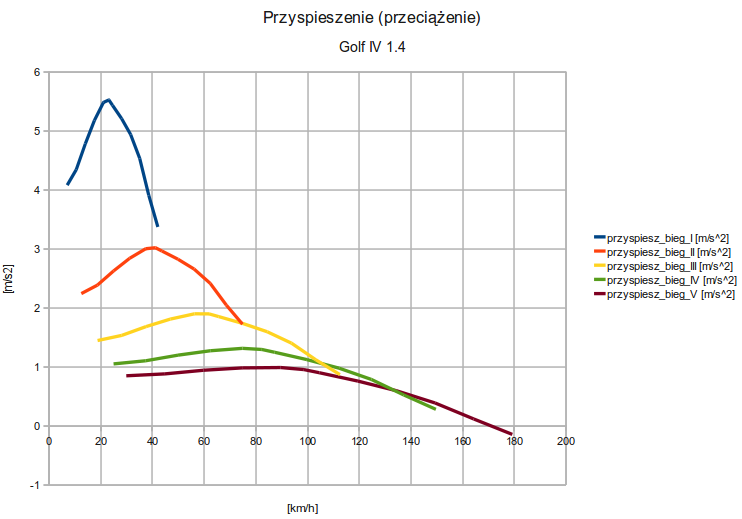
\includegraphics[width=\textwidth,keepaspectratio]{img/golf_acc}
\textit{Przukład charakterystyki przyśpieszenia od prędkości z uwzględnieniem biegów dla Volksvagena Golf IV 1.4. [11].}
\end{center}
}
\par{
Analogicznie sprawa wygląda jeśli chodzi o opóźnienia, które wg. literatury [9] wynoszą $3.0-4.5m/s^2$ dla samochodów w zależności od rodzaju pojazdu jak i stanu nawierzchni. Oraz $6.0-9.8m/s^2$ dla motocykli.
}
\subsubsection{Piesi}
\par{
Charakterystyka pieszych z punktu widzenia ich zewnętrznej obserwacji jest paradoksalnie bardzo zbliżona do charakterystyki DVE. Można bowiem uznać, że świadomość steruje bezpośrednio interfejsem pojazdu, którym staje się ciało ludzkie - wtedy wszystkie złożenia dotyczące DVE zostają aktualne.
}
\par{
Naturalnie piesi mają inną fizyczną dynamikę. I tak przeciętna prędkość pieszego wynosi $~5km/h$ [12] a czas średni czas rozpędzania się do tej prędkości wynosi $~2.25s$ [12]. Oba te prametry stanowią pewne stałe, które mogą być zastosowane dla uproszczenia, jednak źródła [12] podają, iż parametry te zmieniają się w zależności od licznych czynników jak płeć pieszego, dzień tygodnia, rodzaj nawierzchni, pogoda, temperatura itd. Należy uwzględnić istotne z punktu widzenia celu modelowania korelacje.
}